% 圆锥曲线的极坐标方程

\pentry{极坐标的定义\upref{Polar}}

\subsection{结论}
圆锥曲线的极坐标方程为
\begin{equation}
\rho  = \frac{p}{{1 - e\cos \theta }}
\end{equation}
其中 $p$ 是通径, $e$ 是离心率.

\begin{figure}[ht]
\centering
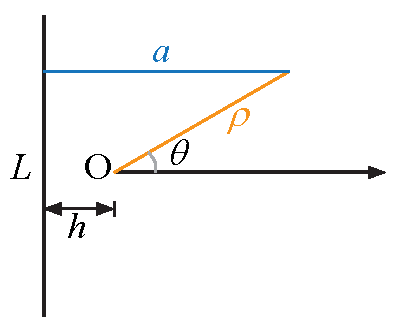
\includegraphics[width=4.5cm]{./figures/Cone1.pdf}
\caption{由离心率定义圆锥曲线}\label{Cone_fig1}
\end{figure}

\subsection{推导}
圆锥曲线的一种定义(与其他定义等效)为(\autoref{Cone_fig1}):
平面上有一点 $O$ 和一条直线 $L$, 相距为 $h$. 
平面上某一点到 $O$ 的距离为 $\rho $, 到 $L$ 的
(垂直)距离为 $a$, 令常数 $e > 0$, 则所有满足
\begin{equation}\label{Cone_eq1}
\rho/a = e
\end{equation}
的点组成的曲线就是圆锥曲线. $e$ 是常数,是\textbf{离心率}, $O$ 是\textbf{焦点}, $L$ 是\textbf{准线}.当 $0 < e < 1$ 时,曲线是椭圆, $e = 1$ 时是抛物线, $e > 1$ 时是双曲线.

以 $O$ 点为原点,使极轴垂直于准线(如上图).则 $a = h + \rho \cos \theta $, 根据\autoref{Cone_eq1} 得
\begin{equation}\label{Cone_eq2}
\frac{\rho }{{h + \rho \cos \theta }} = e
\end{equation}
变形,得
\begin{equation}\label{Cone_eq3}
\rho  = \frac{{eh}}{{1 - e\cos \theta }}
\end{equation}


\begin{figure}[h]
\vskip0pt
\centering
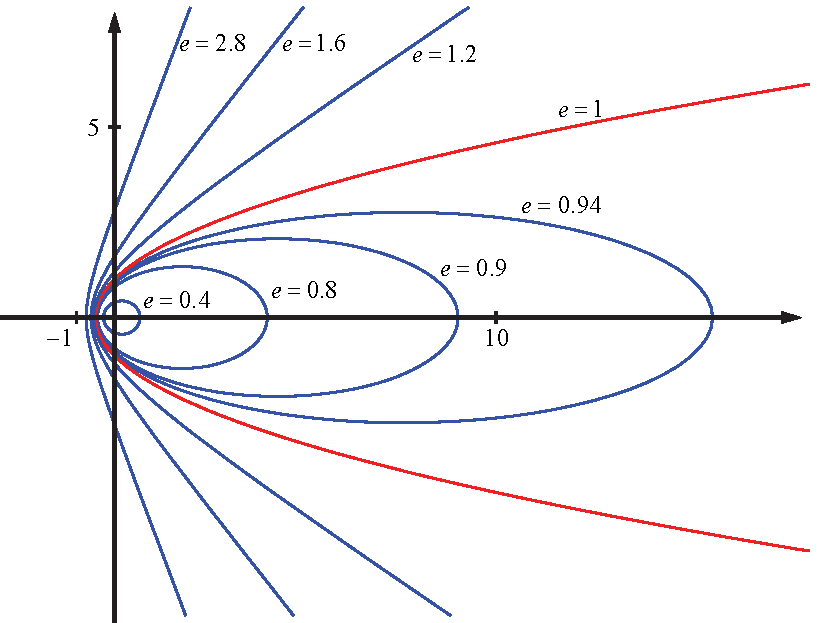
\includegraphics[width=0.8\textwidth]{./figures/Cone2.pdf}
\caption{不同离心率 $e$ 的圆锥曲线}
\vspace{0pt}
\end{figure}
若定义圆锥曲线的\textbf{通径}为过焦点且平行于准线的直线被圆锥曲线截出的线段,令其长度为 $2p$, 那么有 $\rho (\pi /2) = p$. 代入\autoref{Cone_eq3} 得. 所以\autoref{Cone_eq3} 又可以写为
\begin{equation}\label{Cone_eq4}
\rho  = \frac{p}{{1 - e\cos \theta }}
\end{equation}


注意 $p$ 和 $e$ 分别控制圆锥曲线的大小和形状.由于抛物线的 $e = 1$ 不变,所以所有抛物线的形状都相同.

若把曲线围绕焦点顺时针旋转 ${\theta _0}$, 方程就成为
\begin{equation}\label{Cone_eq5}
\rho  = \frac{p}{{1 - e\cos \left( {\theta  + {\theta _0}} \right)}}
\end{equation}
这是更一般的形式.




